%%%%%%%%%%%%%%%%%%%%%%%%%%%%%%%%%%%%%%%%%
% Jacobs Landscape Poster
% LaTeX Template
% Version 1.0 (29/03/13)
%
% Created by:
% Computational Physics and Biophysics Group, Jacobs University
% https://teamwork.jacobs-university.de:8443/confluence/display/CoPandBiG/LaTeX+Poster
% 
% Further modified by:
% Nathaniel Johnston (nathaniel@njohnston.ca)
%
% Modified further still by:
% Abraham Nunes (nunes <at> dal <dot> ca)
%
% License:
% CC BY-NC-SA 3.0 (http://creativecommons.org/licenses/by-nc-sa/3.0/)
%
%%%%%%%%%%%%%%%%%%%%%%%%%%%%%%%%%%%%%%%%%

%----------------------------------------------------------------------------------------
%	PACKAGES AND OTHER DOCUMENT CONFIGURATIONS
%----------------------------------------------------------------------------------------

\documentclass[final]{beamer}
\usepackage{caption}
\usepackage{subcaption}
\usepackage[scale=1,orientation=portrait]{beamerposter} % Use the beamerposter package for laying out the poster

\usetheme{confposter} % Use the confposter theme supplied with this template

\setbeamercolor{block title}{fg=black,bg=white} % Colors of the block titles
\setbeamercolor{block body}{fg=black,bg=white} % Colors of the body of blocks
\setbeamercolor{block alerted title}{fg=white,bg=black} % Colors of the highlighted block titles
\setbeamercolor{block alerted body}{fg=black,bg=five38} % Colors of the body of highlighted blocks
% Many more colors are available for use in beamerthemeconfposter.sty

%-----------------------------------------------------------
% Define the column widths and overall poster size
% To set effective sepwid, onecolwid and twocolwid values, first choose how many columns you want and how much separation you want between columns
% In this template, the separation width chosen is 0.024 of the paper width and a 4-column layout
% onecolwid should therefore be (1-(# of columns+1)*sepwid)/# of columns e.g. (1-(4+1)*0.024)/4 = 0.22
% Set twocolwid to be (2*onecolwid)+sepwid = 0.464
% Set threecolwid to be (3*onecolwid)+2*sepwid = 0.708

% The below is a fix for the lmodern bug with large summation symbols
% declare `cmex` to be arbitrary scalable
\DeclareFontShape{OMX}{cmex}{m}{n}{
  <-7.5> cmex7
  <7.5-8.5> cmex8
  <8.5-9.5> cmex9
  <9.5-> cmex10
}{}

\SetSymbolFont{largesymbols}{normal}{OMX}{cmex}{m}{n}
\SetSymbolFont{largesymbols}{bold}  {OMX}{cmex}{m}{n}
% Bugfix ends here

\newlength{\sepwid}
\newlength{\onecolwid}
\newlength{\twocolwid}
\newlength{\threecolwid}
\setlength{\paperwidth}{24in} % A0 width: 46.8in
\setlength{\paperheight}{36in} % A0 height: 33.1in
\setlength{\sepwid}{0.024\paperwidth} % Separation width (white space) between columns
\setlength{\onecolwid}{0.30\paperwidth} % Width of one column
\setlength{\twocolwid}{0.464\paperwidth} % Width of two columns
\setlength{\threecolwid}{0.708\paperwidth} % Width of three columns
\setlength{\topmargin}{-1in} % Reduce the top margin size
%-----------------------------------------------------------

\usepackage{graphicx}  % Required for including images

\usepackage{booktabs} % Top and bottom rules for tables

%----------------------------------------------------------------------------------------
%	TITLE SECTION 
%----------------------------------------------------------------------------------------
\title{Photometry of Celestial Fireballs} % Poster title

\author{Luke Russell | Willamette University | Advised by Dr.~Jed Rembold} % Author(s)
%----------------------------------------------------------------------------------------

\begin{document}

\addtobeamertemplate{block end}{}{\vspace*{2ex}} % White space under blocks
\addtobeamertemplate{block alerted end}{}{\vspace*{2ex}} % White space under highlighted (alert) blocks

\setlength{\belowcaptionskip}{0ex} % White space under figures
\setlength\belowdisplayshortskip{2ex} % White space under equations

\begin{frame}[t] % The whole poster is enclosed in one beamer frame

\begin{columns}[t] % The whole poster consists of three major columns, the second of which is split into two columns twice - the [t] option aligns each column's content to the top

\begin{column}{\sepwid}\end{column} % Empty spacer column

\begin{column}{.8\twocolwid} % The first column

%----------------------------------------------------------------------------------------
%	OBJECTIVES
%----------------------------------------------------------------------------------------

\setbeamercolor{block alerted title}{fg=white,bg=msblue} % Change the alert block title colors
\setbeamercolor{block alerted body}{fg=black,bg=white} % Change the alert block body colors

\begin{block}{Introduction}

To protect space endeavors, more information is needed about the near-Earth meteoroid population. We created a portable all-sky camera system that hopes to increase the flexibility and affordability of meteoroid observation systems. This project focused on writing software perform accurate photometric data reduction.

\end{block}

\begin{alertblock}{Objectives}

 \begin{itemize}
\item Create a program that can analyze moving photometric data from meteor video
\item Test program on known events to test its accuracy and validity
\item Use program to analyze events captured by our own all-sky camera
\end{itemize}

\end{alertblock}


\begin{alertblock}{Our All-Sky Camera}

\begin{figure}
\centering
\begin{subfigure}{.7\textwidth}
  \centering
  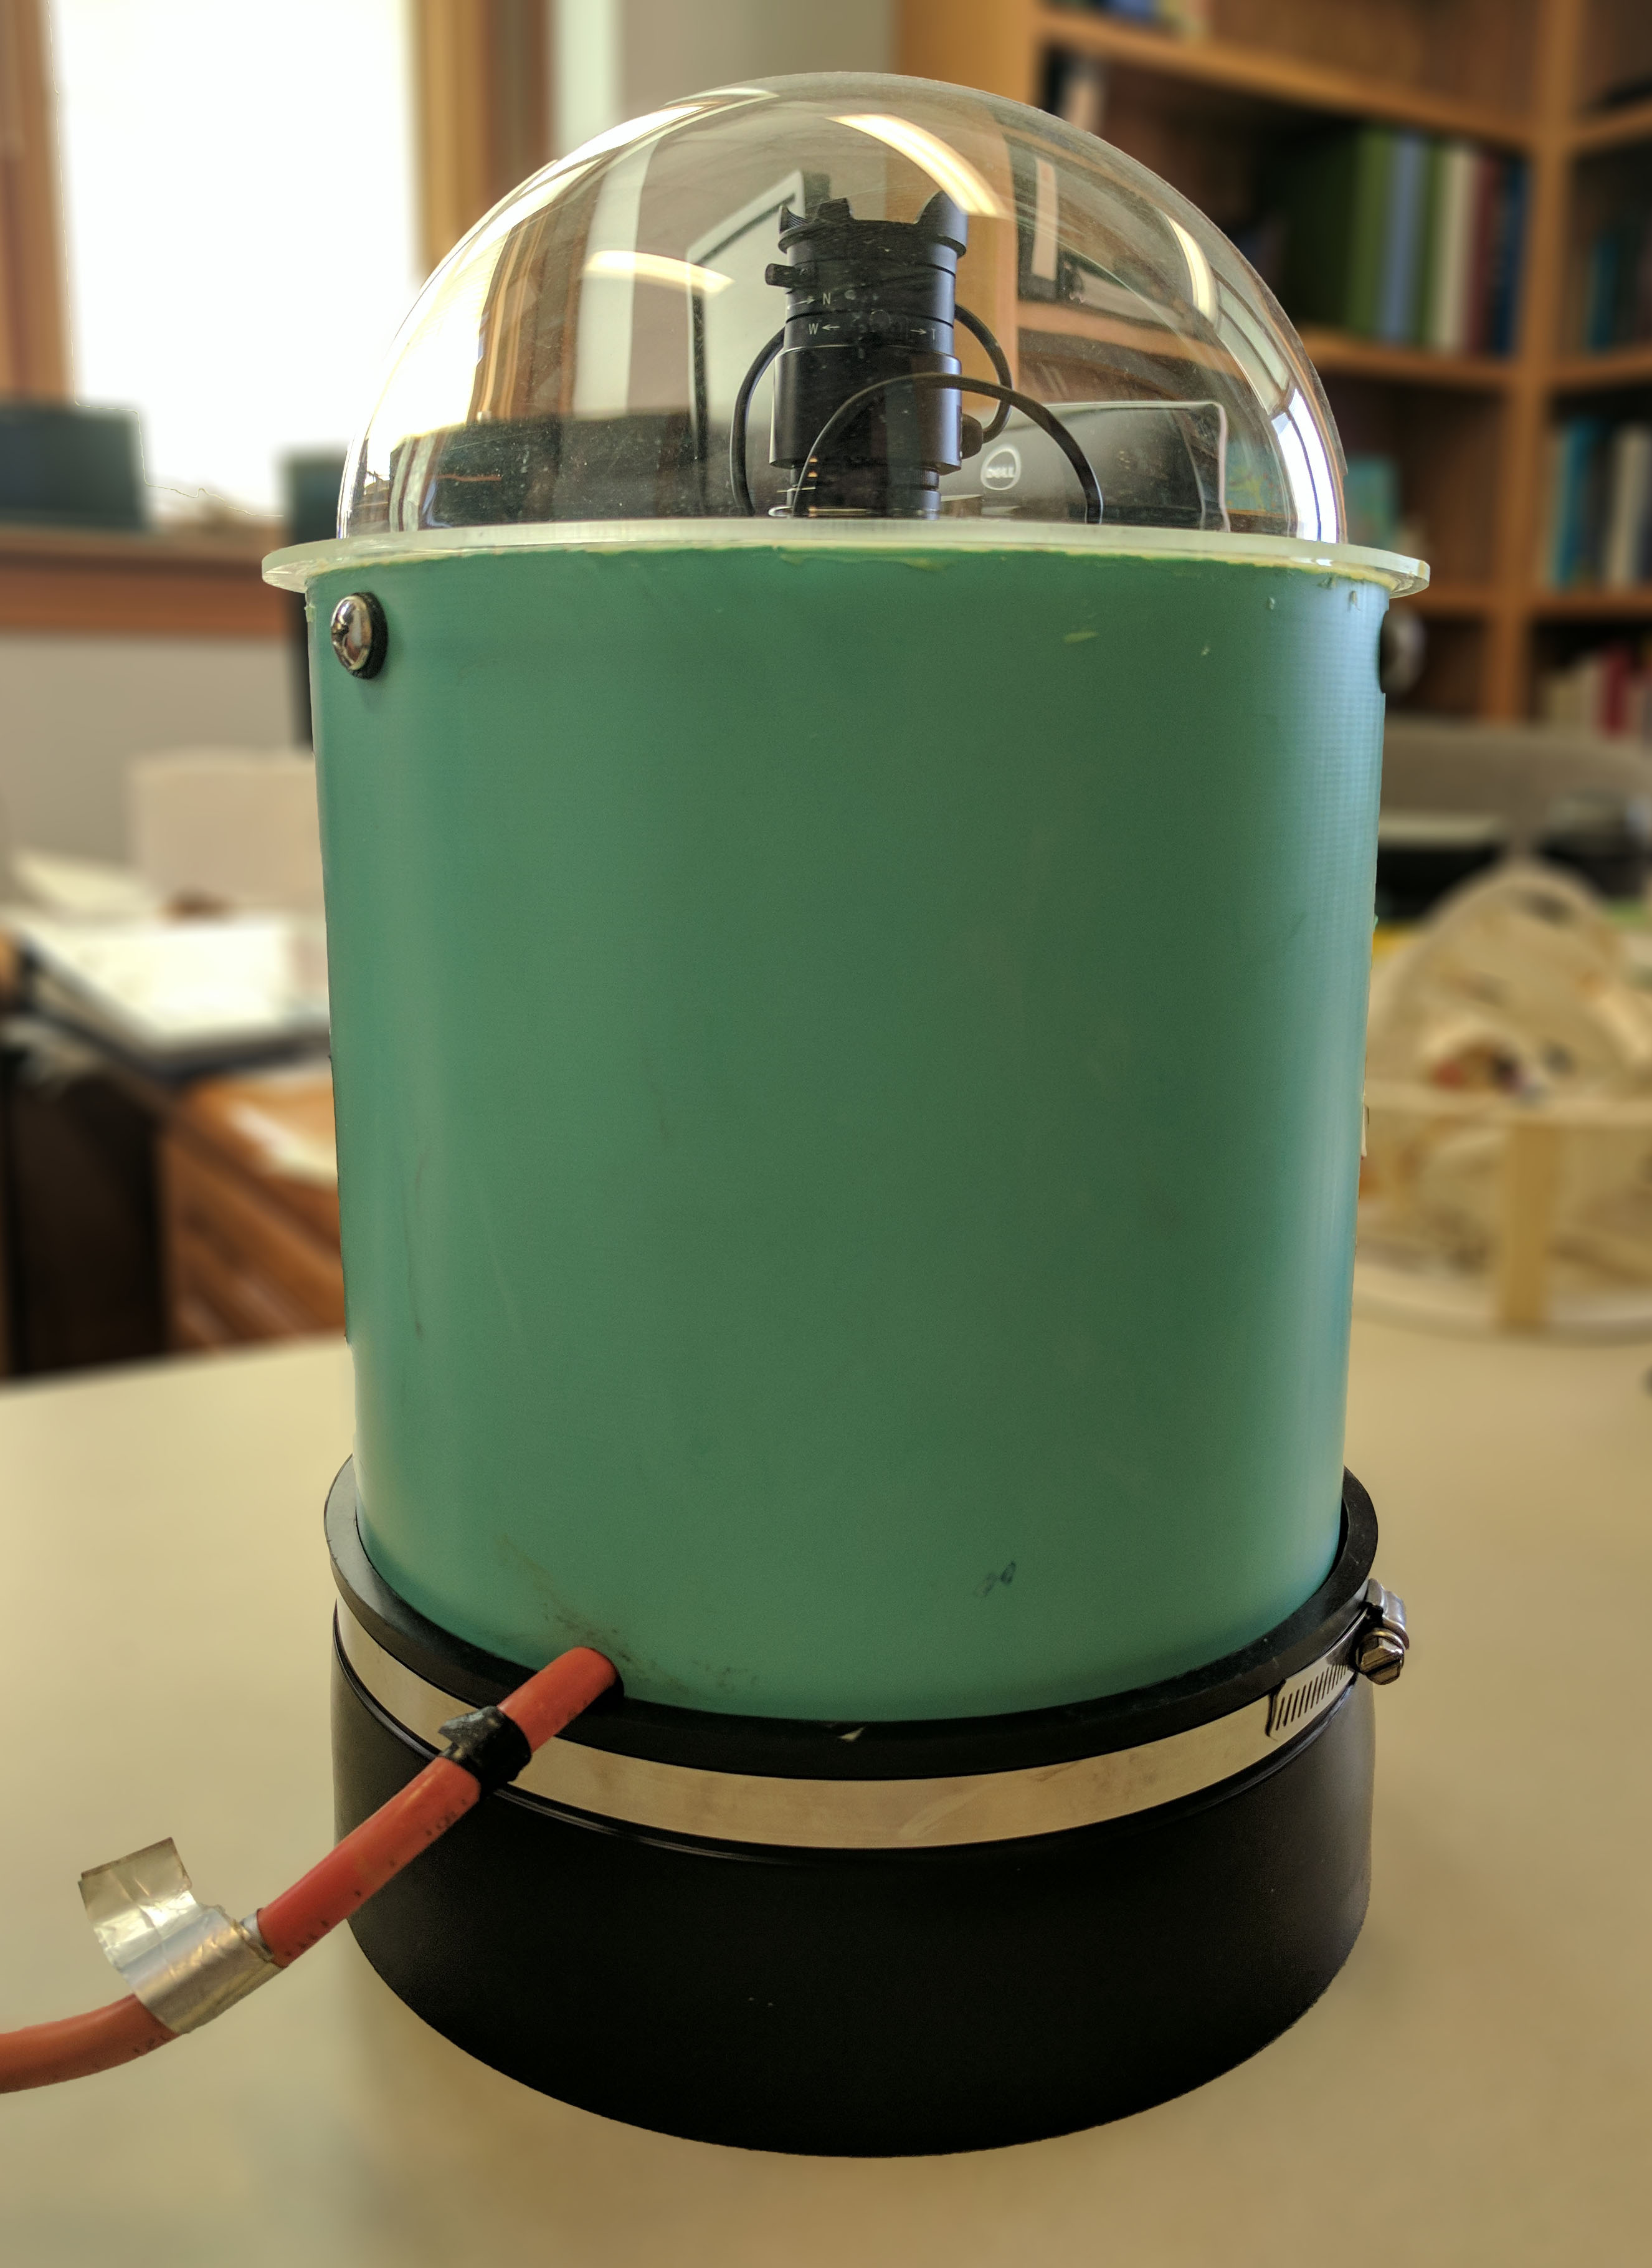
\includegraphics[width=\linewidth]{deesix.jpg}
  \label{fig:d6}
\end{subfigure}%
%\begin{subfigure}{0\textwidth}
  %\centering
  %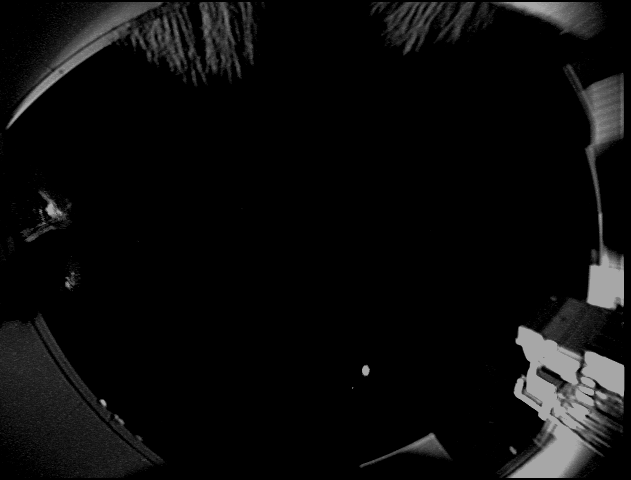
\includegraphics[width=\linewidth]{iridium3.png}
  %\label{fig:sub2}
%\end{subfigure}
\end{figure}

\end{alertblock}
%------------------------------------------------
\begin{block}{Mathematical Methods}

	Our camera reports light \textbf{intensity} as an 8-bit integer value, ranging from 0 to 255. Summing over the intensity values for each pixel in an event approximates the total intensity of the event. We use Equation~\ref{eqn:Light} to turn that into an uncalibrated \textbf{magnitude}, which is a log scale and generally how astronomical brightnesses are reported. 
\begin{equation}
	m = -2.5 \log\Big(\sum_{pixels} I\Big)
\label{eqn:Light}
\end{equation}

This magnitude is uncalibrated however, and measurements from different systems would disagree as to its value. The system is calibrated by observing a star of known magnitude during the event. This yields a correction factor needed to relate the sum of the pixels to the known magnitude. This correction factor is then applied to the unknown magnitude to determine the calibrated apparent magnitude of the event.

%From intensity, we can extrapolate out to get the object's total \textbf{luminosity}. We can then relate the luminosity of the event to its total \textbf{kinetic energy} to find its \textbf{mass} through integration of its light curve,

%\begin{equation}
%L = \tau \frac{v^1}{2} \frac{dM}{dt}
%\label{eq:Mass}
%\end{equation}
\end{block}
%----------------------------------------------------------------------------------------

\end{column} % End of the first column

\begin{column}{\sepwid}\end{column} % Empty spacer column

\begin{column}{1.2\twocolwid} % Begin a column which is two columns wide (column 2)
\setbeamercolor{block alerted title}{fg=white,bg=msblue} % Change the alert block title colors
\setbeamercolor{block alerted body}{fg=black,bg=five38} % Change the alert block body colors

\begin{alertblock}{Analysis Procedure}

\begin{figure}
\centering
\begin{subfigure}{.5\textwidth}
  \centering
  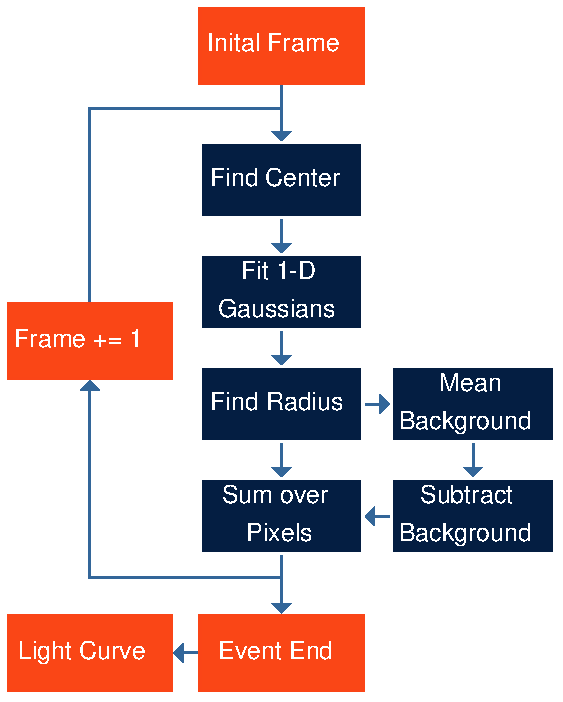
\includegraphics[width=\linewidth]{flowchartastro.pdf}
  \label{fig:flowchart}
\end{subfigure}%
\begin{subfigure}{.5\textwidth}
  \centering
  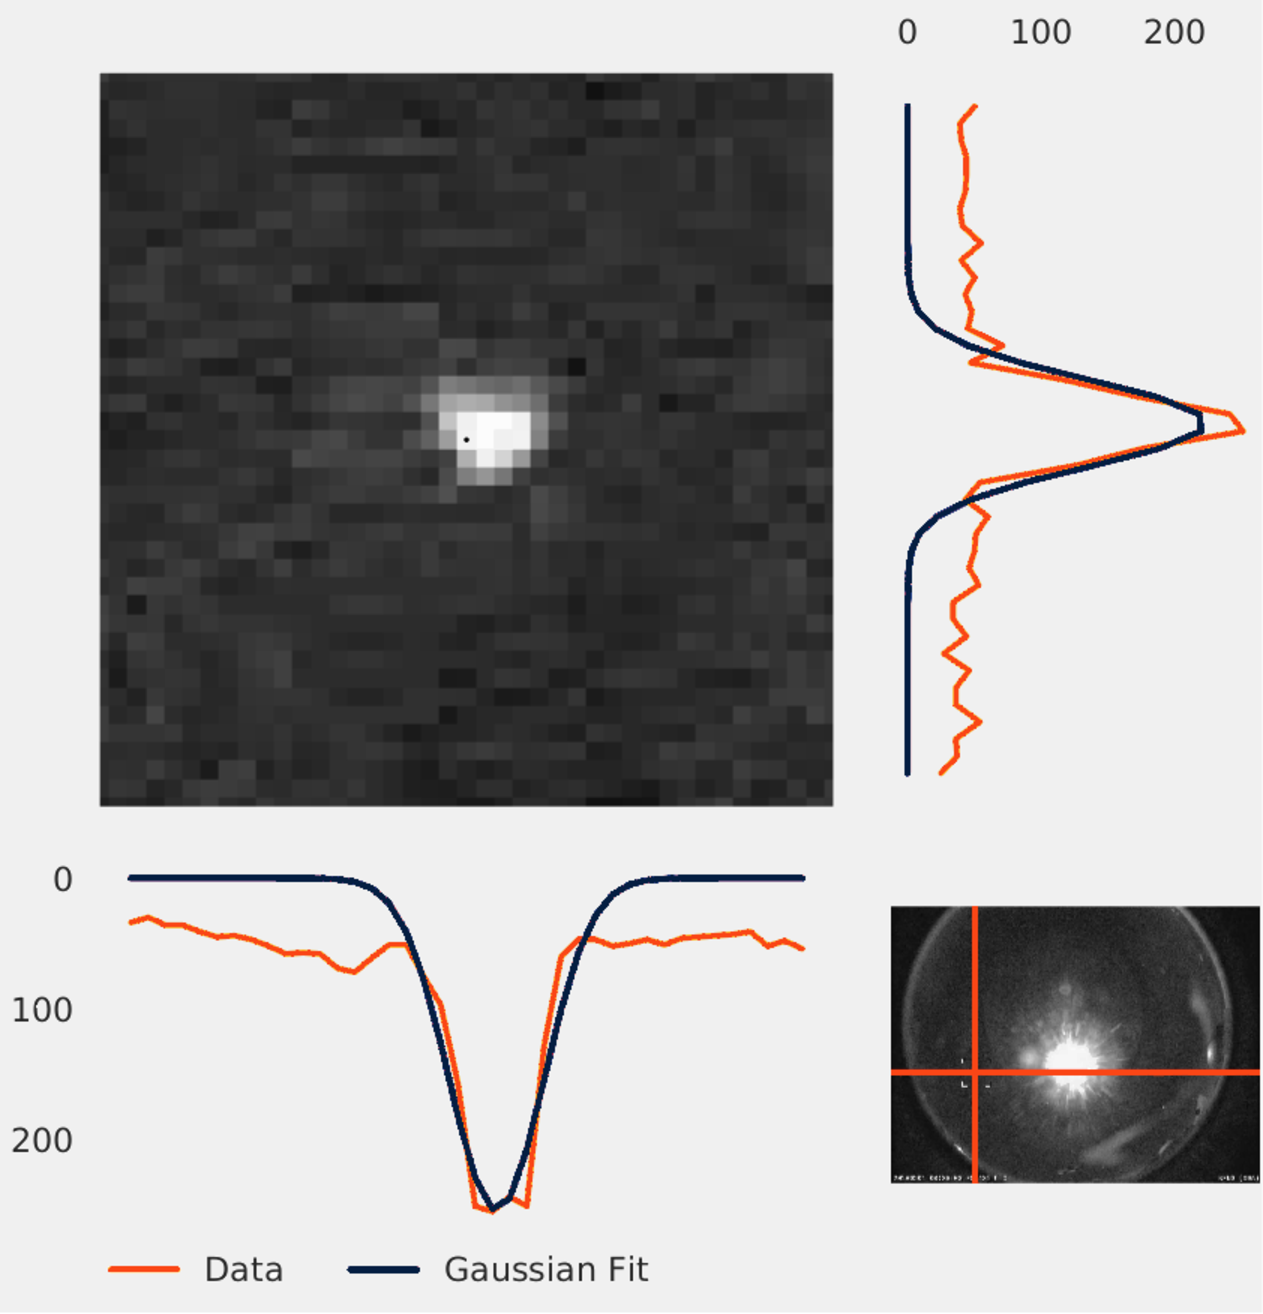
\includegraphics[width=\linewidth]{testplot3.pdf}
  \label{fig:gaussians}
\end{subfigure}
\end{figure}
\vspace{-2cm}
\end{alertblock}

%\begin{block}{Computational Methods}
\setbeamercolor{block alerted title}{fg=white,bg=msblue} % Change the alert block title colors
\setbeamercolor{block alerted body}{fg=black,bg=white} % Change the alert block body colors

\begin{alertblock}{Photometry Program}
\begin{figure}
	\centering
	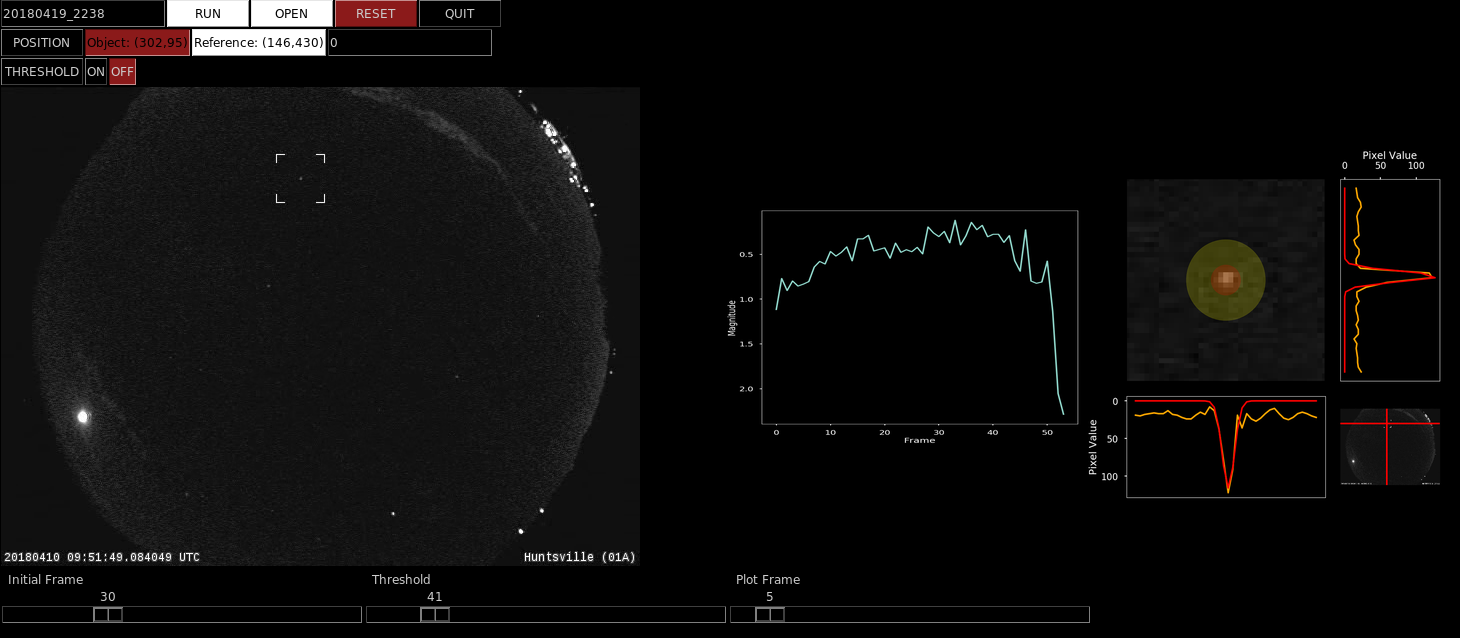
\includegraphics[width=\linewidth]{ProgramLandscape.png}
	\label{fig:}
\end{figure}
\vspace{-1.5cm}
\end{alertblock}
%\end{block}


%----------------------------------------------------------------------------------------
%	RESULTS
%----------------------------------------------------------------------------------------

\setbeamercolor{block alerted title}{fg=white,bg=msyellow} % Change the alert block title colors
\setbeamercolor{block alerted body}{fg=black,bg=five38} % Change the alert block body colors


\begin{block}{Results}
As a test, the program was run on meteor events collected by NASA's ASGARD all-sky network. Lightcurves are also available for this data, and serve as a useful comparison and analysis check. On all comparisons thus far the program has compared favorably. 
\end{block}

\begin{alertblock}{Meteor Data}

\begin{figure}
\centering
\begin{subfigure}{.52\textwidth}
  \centering
  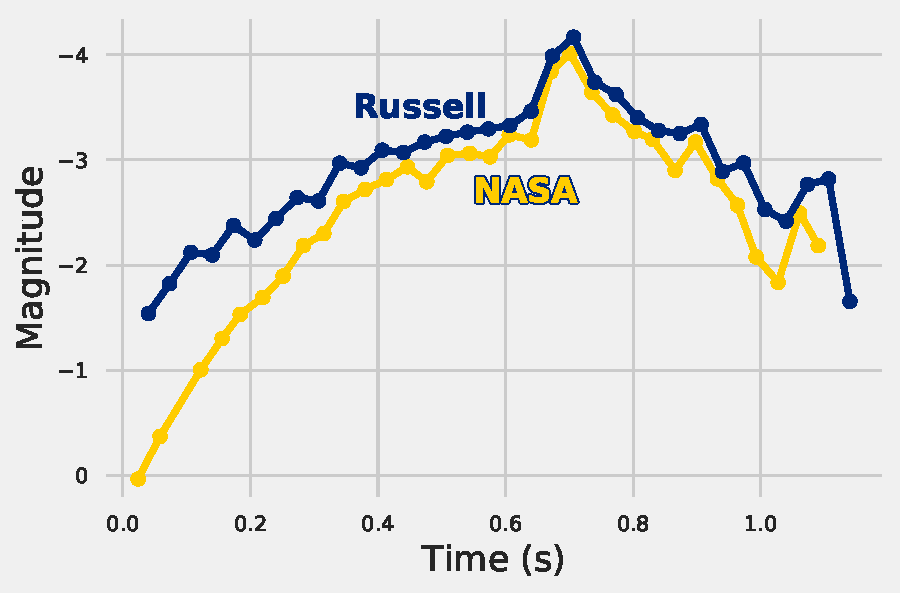
\includegraphics[width=\linewidth]{PosterGraph.pdf}
  \label{fig:sub1}
\end{subfigure}%
\begin{subfigure}{.48\textwidth}
  \centering
  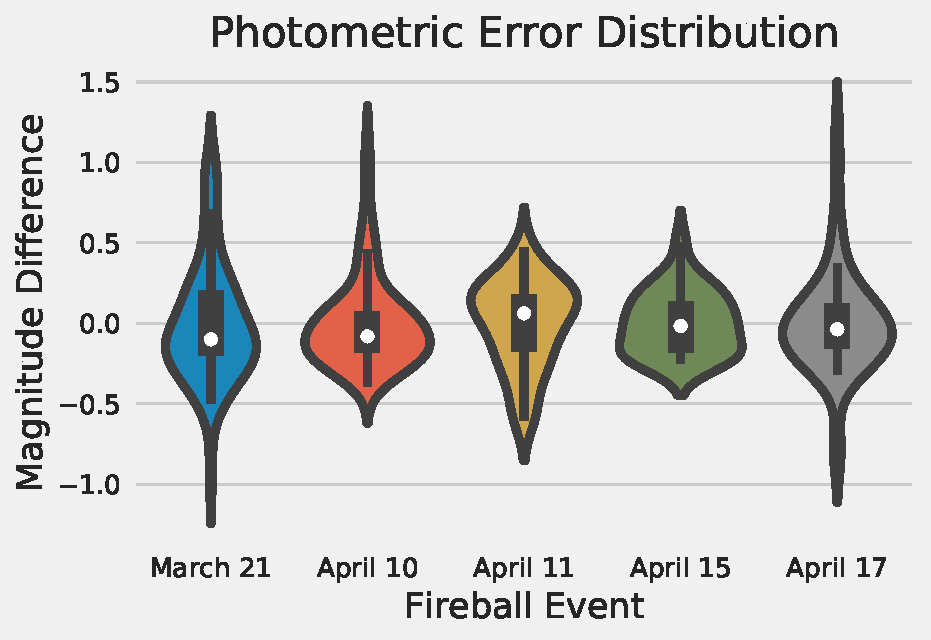
\includegraphics[width=\linewidth]{theviolinplot.pdf}
  \label{fig:sub2}
\end{subfigure}
\label{fig:test}
\end{figure}
\vspace{-1.5cm}
\end{alertblock}

\vspace{-1cm}
%\vspace{-1.5cm}

%----------------------------------------------------------------------------------------
%	CONCLUSION
%----------------------------------------------------------------------------------------


\begin{block}{Conclusion}

The photometric program we wrote appears to be successful at finding the calibrated magnitudes of events. There is some fine tweaking and optimization to be done, but after that, it is onto collecting enough data to statistically analyze and create our own population distribution of meteoroids. 

\end{block}


%----------------------------------------------------------------------------------------
%	REFERENCES
%----------------------------------------------------------------------------------------

%\begin{block}{References}

%\nocite{*} % Insert publications even if they are not cited in the poster
%\small{\bibliographystyle{unsrt}
%\bibliography{sample}\vspace{0.75in}}

%\end{block}

%----------------------------------------------------------------------------------------
%	ACKNOWLEDGEMENTS
%----------------------------------------------------------------------------------------

\setbeamercolor{block title}{fg=black,bg=white} % Change the block title color

%\begin{block}{Acknowledgements}

%\small{\rmfamily{Nam mollis tristique neque eu luctus. Suspendisse rutrum congue nisi sed convallis. Aenean id neque dolor. Pellentesque habitant morbi tristique senectus et netus et malesuada fames ac turpis egestas.}} \\

%\end{block}

%----------------------------------------------------------------------------------------
%	CONTACT INFORMATION
%----------------------------------------------------------------------------------------

\setbeamercolor{block alerted title}{fg=black,bg=dalblue} % Change the alert block title colors
\setbeamercolor{block alerted body}{fg=black,bg=five38} % Change the alert block body colors

%\begin{alertblock}{Contact Information}

%\begin{itemize}
%\item Web: Github.com/LukeGalbraithRussell
%\item Email: lgrussel@Willamette.edu
%\end{itemize}

%\end{alertblock}

%\begin{center}
%
\includegraphics[width=0.8\linewidth]{dal_fullmark_blak.jpg}
%\end{center}
%----------------------------------------------------------------------------------------

\end{column} % End of the third column

\end{columns} % End of all the columns in the poster

\end{frame} % End of the enclosing frame

\end{document}
